Si 

\begin{equation}
    A = 
    \begin{pmatrix}
     7 &  3 & -1 &  2 \\ 
     3 &  8 &  1 & -4 \\
    -1 &  1 &  4 & -1 \\
     2 & -4 & -1 &  6
    \end{pmatrix}
    , \quad \quad
    b = 
    \begin{pmatrix}
    -1 \\ 
     0 \\
    -3 \\
     1
    \end{pmatrix}
\end{equation}

Para  el  sistema  $Ax=b$:

\begin{itemize}
    \item Use los  métodos  iterativos  de  Jacobi,  Gauss-Seidel y  SOR  con  valor  de $\omega=1.4$, escriba  y  ejecute  un  código para  resolver  el  sistema  lineal con  cuatro  decimales  de  precisión,  compare  el  número de  iteraciones  en  cada  caso.
    \item Resuelva  usando  el  método  de  SOR,  con $\omega=1.1$;  $\omega=1.3$;  $\omega=1.8$;  luego  trace  la  gráfica  del  numero  de  iteraciones  para  la  convergencia  contra  los  valores de $\omega$, ¿Qué valor  da  como  resultado la  convergencia  más rápida?
\end{itemize}

\textbf{Solución:}

\begin{itemize}
\item Resolviendo el problema por el método de Jacobi:

%\begin{table}[h]
    \begin{center}
    \begin{tabular}{r|llll}
        Iteración & $x_0$ & $x_1$ & $x_2$ & $x_3$ \\
        \hline
        0 & 0 & 0 & 0 & 0 \\
        1 & -0.14286 & 0.00000 & -0.75000 & 0.16667 \\
        2 & -0.29762 & 0.23065 & -0.74405 & 0.08929 \\
        3 & -0.37351 & 0.24926 & -0.85975 & 0.29563 \\
        4 & -0.45697 & 0.39535 & -0.83178 & 0.31405 \\
        5 & -0.52085 & 0.43236 & -0.88457 & 0.44393 \\
        6 & -0.58136 & 0.52785 & -0.87732 & 0.48110 \\
        7 & -0.63187 & 0.56822 & -0.90703 & 0.56613 \\
        8 & -0.67771 & 0.63340 & -0.90849 & 0.60493 \\
        9 & -0.71693 & 0.67017 & -0.92654 & 0.66342 \\
        10 & -0.75198 & 0.71638 & -0.93092 & 0.69800 \\
        11 & -0.78229 & 0.74736 & -0.94259 & 0.73976 \\
        12 & -0.80917 & 0.78106 & -0.94747 & 0.76857 \\
        13 & -0.83254 & 0.80616 & -0.95542 & 0.79919 \\
        14 & -0.85318 & 0.83122 & -0.95988 & 0.82238 \\
        15 & -0.87119 & 0.85112 & -0.96551 & 0.84523 \\
        16 & -0.88705 & 0.87000 & -0.96927 & 0.86356 \\
        17 & -0.90091 & 0.88558 & -0.97337 & 0.88080 \\
        18 & -0.91310 & 0.89992 & -0.97642 & 0.89513 \\
        19 & -0.92378 & 0.91203 & -0.97947 & 0.90824 \\
        20 & -0.93315 & 0.92297 & -0.98189 & 0.91937 \\
        21 & -0.94136 & 0.93235 & -0.98419 & 0.92938 \\
        22 & -0.94857 & 0.94072 & -0.98608 & 0.93799 \\
        23 & -0.95489 & 0.94797 & -0.98783 & 0.94566 \\
        24 & -0.96044 & 0.95439 & -0.98930 & 0.95231 \\
        25 & -0.96530 & 0.95998 & -0.99063 & 0.95819 \\
        26 & -0.96956 & 0.96491 & -0.99177 & 0.96331 \\
        27 & -0.97330 & 0.96921 & -0.99279 & 0.96783 \\
        28 & -0.97659 & 0.97300 & -0.99367 & 0.97178 \\
        29 & -0.97946 & 0.97632 & -0.99445 & 0.97525 \\
        30 & -0.98199 & 0.97923 & -0.99513 & 0.97829 \\
        31 & -0.98420 & 0.98178 & -0.99573 & 0.98096 \\
        32 & -0.98614 & 0.98402 & -0.99626 & 0.98330 \\
    \end{tabular}
    \end{center}

\begin{center}
    \begin{tabular}{r|llll}
        Iteración & $x_0$ & $x_1$ & $x_2$ & $x_3$ \\
        \hline
        33 & -0.98785 & 0.98599 & -0.99672 & 0.98535 \\
        34 & -0.98934 & 0.98771 & -0.99712 & 0.98715 \\
        35 & -0.99065 & 0.98922 & -0.99747 & 0.98873 \\
        36 & -0.99180 & 0.99054 & -0.99778 & 0.99012 \\
        37 & -0.99281 & 0.99171 & -0.99806 & 0.99133 \\
        38 & -0.99369 & 0.99273 & -0.99830 & 0.99240 \\
        39 & -0.99447 & 0.99362 & -0.99851 & 0.99333 \\
        40 & -0.99515 & 0.99440 & -0.99869 & 0.99415 \\
        41 & -0.99574 & 0.99509 & -0.99885 & 0.99487 \\
        42 & -0.99627 & 0.99570 & -0.99899 & 0.99550 \\
        43 & -0.99673 & 0.99622 & -0.99912 & 0.99605 \\
        44 & -0.99713 & 0.99669 & -0.99922 & 0.99654 \\
        45 & -0.99748 & 0.99710 & -0.99932 & 0.99696 \\
        46 & -0.99779 & 0.99745 & -0.99940 & 0.99734 \\
        47 & -0.99806 & 0.99777 & -0.99948 & 0.99766 \\
        48 & -0.99830 & 0.99804 & -0.99954 & 0.99795 \\
        49 & -0.99851 & 0.99828 & -0.99960 & 0.99820 \\
        50 & -0.99869 & 0.99849 & -0.99965 & 0.99842 \\
        51 & -0.99885 & 0.99868 & -0.99969 & 0.99862 \\
        52 & -0.99899 & 0.99884 & -0.99973 & 0.99879 \\
        53 & -0.99912 & 0.99898 & -0.99976 & 0.99894 \\
        54 & -0.99923 & 0.99911 & -0.99979 & 0.99907 \\
        55 & -0.99932 & 0.99922 & -0.99982 & 0.99918 \\
        56 & -0.99940 & 0.99931 & -0.99984 & 0.99928 \\
        57 & -0.99948 & 0.99940 & -0.99986 & 0.99937 \\
        58 & -0.99954 & 0.99947 & -0.99988 & 0.99945 \\
        59 & -0.99960 & 0.99954 & -0.99989 & 0.99952 \\
        60 & -0.99965 & 0.99959 & -0.99990 & 0.99958 \\
        61 & -0.99969 & 0.99964 & -0.99992 & 0.99963 \\
        62 & -0.99973 & 0.99969 & -0.99993 & 0.99967 \\
        63 & -0.99976 & 0.99973 & -0.99994 & 0.99971 \\
        64 & -0.99979 & 0.99976 & -0.99994 & 0.99975 \\
        65 & -0.99982 & 0.99979 & -0.99995 & 0.99978 \\
        66 & -0.99984 & 0.99982 & -0.99996 & 0.99981 \\
    \end{tabular}
    \end{center}

Resolviendo el problema por el método de Gauss-Seidel:

\begin{center}
    \begin{tabular}{r|llll}
        Iteración & $x_0$ & $x_1$ & $x_2$ & $x_3$ \\
        \hline
        0 & 0.00000 & 0.00000 & 0.00000 & 0.00000 \\
        1 & -0.14286 & 0.05357 & -0.79911 & 0.11682 \\
        2 & -0.31335 & 0.27580 & -0.86808 & 0.31030 \\
        3 & -0.47373 & 0.44131 & -0.90118 & 0.46859 \\
        4 & -0.59461 & 0.56992 & -0.92399 & 0.59082 \\
        5 & -0.68791 & 0.66888 & -0.94149 & 0.68497 \\
        6 & -0.75972 & 0.74507 & -0.95496 & 0.75746 \\
        7 & -0.81501 & 0.80373 & -0.96532 & 0.81327 \\
        8 & -0.85758 & 0.84889 & -0.97330 & 0.85624 \\
        9 & -0.89035 & 0.88366 & -0.97944 & 0.88932 \\
        10 & -0.91558 & 0.91043 & -0.98417 & 0.91479 \\
        11 & -0.93501 & 0.93104 & -0.98782 & 0.93439 \\
        12 & -0.94996 & 0.94691 & -0.99062 & 0.94949 \\
        13 & -0.96148 & 0.95913 & -0.99278 & 0.96111 \\
        14 & -0.97034 & 0.96853 & -0.99444 & 0.97006 \\
        15 & -0.97717 & 0.97577 & -0.99572 & 0.97695 \\
        16 & -0.98242 & 0.98135 & -0.99670 & 0.98225 \\
        17 & -0.98646 & 0.98564 & -0.99746 & 0.98634 \\
        18 & -0.98958 & 0.98894 & -0.99805 & 0.98948 \\
        19 & -0.99198 & 0.99149 & -0.99850 & 0.99190 \\
        20 & -0.99382 & 0.99345 & -0.99884 & 0.99377 \\
        21 & -0.99524 & 0.99495 & -0.99911 & 0.99520 \\
        22 & -0.99634 & 0.99612 & -0.99931 & 0.99630 \\
        23 & -0.99718 & 0.99701 & -0.99947 & 0.99715 \\
        24 & -0.99783 & 0.99770 & -0.99959 & 0.99781 \\
        25 & -0.99833 & 0.99823 & -0.99969 & 0.99831 \\
        26 & -0.99871 & 0.99864 & -0.99976 & 0.99870 \\
        27 & -0.99901 & 0.99895 & -0.99981 & 0.99900 \\
        28 & -0.99924 & 0.99919 & -0.99986 & 0.99923 \\
        29 & -0.99941 & 0.99938 & -0.99989 & 0.99941 \\
        30 & -0.99955 & 0.99952 & -0.99992 & 0.99954 \\
        31 & -0.99965 & 0.99963 & -0.99993 & 0.99965 \\
        32 & -0.99973 & 0.99972 & -0.99995 & 0.99973 \\
        33 & -0.99979 & 0.99978 & -0.99996 & 0.99979 \\
        34 & -0.99984 & 0.99983 & -0.99997 & 0.99984 \\
        35 & -0.99988 & 0.99987 & -0.99998 & 0.99988 \\
        36 & -0.99991 & 0.99990 & -0.99998 & 0.99990 \\
        37 & -0.99993 & 0.99992 & -0.99999 & 0.99993 \\
    \end{tabular}
    \end{center}

Resolviendo el problema por el método SOR  con  $\omega=1.4$:

    \begin{center}
    \begin{tabular}{r|llll}
        Iteración & $x_0$ & $x_1$ & $x_2$ & $x_3$ \\
        \hline
        0 & 0 & 0 & 0 & 0 \\
        1 & -0.200000 & 0.105000 & -1.156750 & 0.154758 \\
        2 & -0.476253 & 0.518795 & -0.881402 & 0.672230 \\
        3 & -0.765948 & 0.819411 & -1.017035 & 0.849359 \\
        4 & -0.928418 & 0.932188 & -0.997122 & 0.964231 \\
        5 & -0.973062 & 0.987441 & -0.999846 & 0.990051 \\
        6 & -0.999229 & 0.997628 & -1.002444 & 1.000836 \\
        7 & -0.999708 & 1.001808 & -0.999261 & 1.001389 \\
        8 & -1.001610 & 1.000965 & -1.000711 & 1.000930 \\
        9 & -1.000449 & 1.000625 & -0.999766 & 1.000476 \\
        10 & -1.000339 & 1.000220 & -1.000123 & 1.000145 \\
        11 & -1.000079 & 1.000076 & -0.999955 & 1.000061 \\zz
        12 & -1.000029 & 1.000019 & -1.000014 & 1.000004 \\
        13 & -1.000004 & 1.000000 & -0.999994 & 1.000002 \\
    \end{tabular} \\
    \end{center}

\item Hacemos uso del método SOR con $\omega=1.1$ (convergencia con 68 iteraciones);  $\omega=1.3$ (convergencia con 38 iteraciones);  $\omega=1.8$ (convergencia con 110 iteraciones).

\begin{figure}[h]
    \centering
    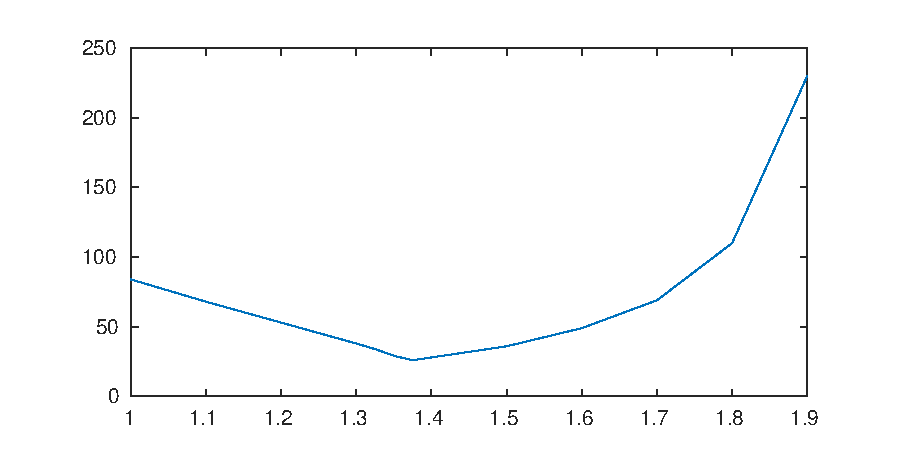
\includegraphics[scale=0.8]{Adicionales/iteraciones.eps} 
    \caption{Número de iteración necesarios para alcanzar convergencia al usar el método SOR, con respecto al valor $\omega$.}
    \label{test0}
\end{figure}


% 1.0 -> 84
% 1.1 -> 68
% 1.2 -> 53
% 1.3 -> 38
% 1.3511 -> 13
% 1.4 -> 28
% 1.5-> 36
% 1.6-> 49
% 1.7-> 69
% 1.8 -> 110
% 1.9 -> 230

%w = [1:0.1:1.3 1.325 1.3511 1.375 1.4:0.1:1.9];
%itr =[84 68 53 38 34 29 26 28 36 49 69 110 230];

\end{itemize}
